\chapter{Overview of JavaScript and V8 engine architecture}
\label{cha:overview}

Historically, JavaScript was considered untyped language, meaning that values had no types attached to variables, either by programmer or compiler. All variables were of single, unified type and procedures called unboxing and boxing, performed before and after each operation on variable, ensured that it was properly used on machine code level. Complete code source was sent from server to the browser and was parsed and executed on fly. Without types attached to variables, all functions were polymorphic and unstable, since parameters may have carried any type of variable. To solve this problem source code of function was parsed each time it was called, each time generating machine code based on current parameters and variables in scope. This approach, called interpretation, is still present in JavaScript engines and used whenever variables don't match set criteria of stability described later in this chapter.

This paper uses as an engine of choice V8 Crankshaft. Choice was made because it's the only engine available at the moment which provides direct command line access, enabling precise performance measurements of code parsing and execution, without browser context and overhead. Executable file of V8 (named d8) is compiled with consideration of target platform.

\section{JIT compilation -- tracking variable types}
\label{sec:JIT}

As mentioned before, initially JavaScript was treated as untyped language. With release of SpiderMonkey in Firefox 3.5 in 2009 situation has changed. First Just-In-Time compiler for JavaScript, TraceMonkey, was created. Based on works of Prof. Dr. Michael Franz on TraceTrees \footnote{http://www.michaelfranz.com/} JIT compiler was collecting all paths that interpreter took with specific types of variables. A path could split to different methods or if statements. Whenever part of code was executed often enough, path was marked as hot and compiler optimised it for given types. If single path was traversed with different set of types compiler could generate another version of optimised code. When path tuned out to be highly polymorphic optimised versions were removed and interpreter was used as a fallback.
Initial reports shown speedups between 20x to 40x \footnote{http://arstechnica.com/information-technology/2008/08/firefox-to-get-massive-javascript-performance-boost/}.
However, trace JIT turned out to be very complicated to maintain \footnote{https://hacks.mozilla.org/2010/03/improving-javascript-performance-with-jagermonkey/} and eventually was removed from Firefox in 2011.\footnote{http://blog.mozilla.org/nnethercote/2011/11/23/memshrink-progress-report-week-23/}. At the time SpiderMonkey was already equipped with JägerMonkey, JIT engine based on method calls. Instead of collecting complete traces, only method calls are counted. This gives easy track of function parameters and variables in scope.

\begin{figure}[h!]
  \caption{JIT compiler tracking method calls}
  \label{img:jit-1}
  \centering
	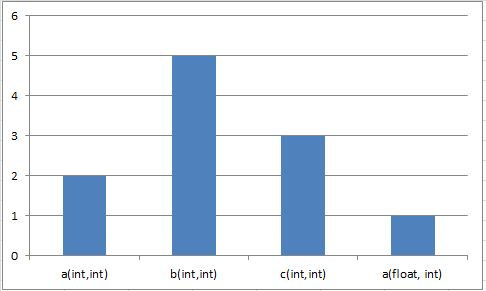
\includegraphics[width=8cm]{jit-1}
\end{figure}


\begin{figure}[h!]
  \caption{JIT compiler marking one of methods as hot and recompiling}
  \label{img:jit-2}
  \centering
	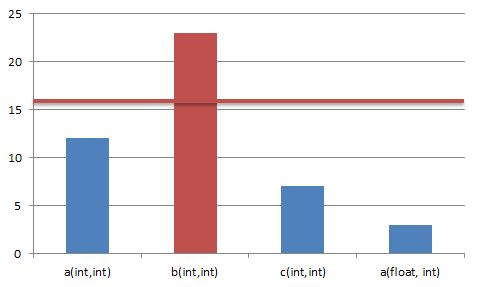
\includegraphics[width=8cm]{jit-2}
\end{figure}

This proved to be more effective and simpler approach and now used in all JavaScript engines. In V8 Crankshaft step forward was taken and simple methods are compiled even before any statistics on data types are collected. For compiled methods source code is not stored. Instead procedure called deoptimisation is implemented. Whenever engine detects that compiled code doesn't match actual types of variables, code is deoptimised and either optimised again to match new, better set of variables, or kept in interpreter friendly form.

To track these changes two debug options for V8 are available: --trace-opt and --trace-deopt.

\lstinputlisting[caption=Output from V8 debug run showing optimisation and deoptimisation,label=listing:optdeopt]{optdeopt.txt}


\section{Type interference}
\label{sec:typeinterference}

V8's method of optimising code before it's run relies on type inference. Based on context of variable it's type is guessed. Generated assembler has to support cache miss -- whenever inferred type turns out to be incorrect, new type is assigned and another JIT compilation runs. Types of variables are organised in a tree, where Number object may store both Float or Integer, Integer may store SMI (small int), etc.

\lstinputlisting[caption=Tree of types in JavaScript,label=listing:typestree]{types.txt}

In V8 type inference is tightly connected with JIT compilation and may be tracked with the same flags: --trace-opt and --trace-deopt. 

\section{Hidden classes}
\label{sec:hiddenclasses}

TODO: add paragraph on dictionary mode in objects.

JavaScript is classless language. Object may have defined a prototype which behaves similar to base class in other langauges. However, a property may be added to an Object or it's prototype at any point in runtime. To optimise such dynamic representation engines use a concept of hidden class. Whenever an Object is created it's hidden class is pointed to base, empty Object representation. Then each definition of new property makes a transition on hidden class graph, introducing hidden classes that are not yet defined, as in following example:

\begin{figure}[h!]
  \caption{Initial shape of hidden class for Point}
  \label{img:point0}
  \centering
	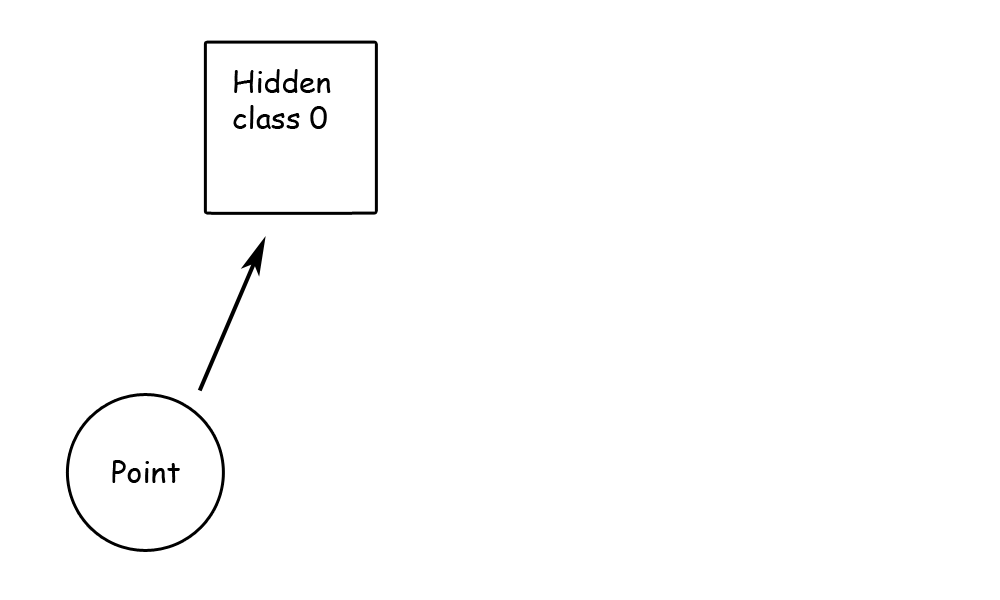
\includegraphics[width=8cm]{point0}
\end{figure}
\begin{figure}[h!]
  \caption{Shape of hidden class for Point after x property added}
  \label{img:point1}
  \centering
	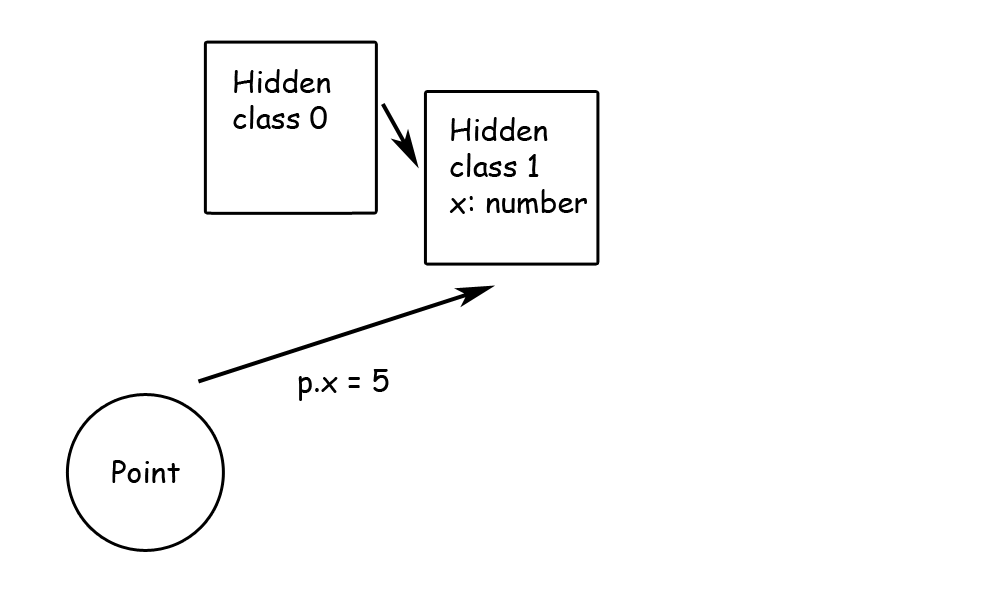
\includegraphics[width=8cm]{point1}
\end{figure}
\begin{figure}[h!]
  \caption{Shape of hidden class for Point after y property added}
  \label{img:point2}
  \centering
	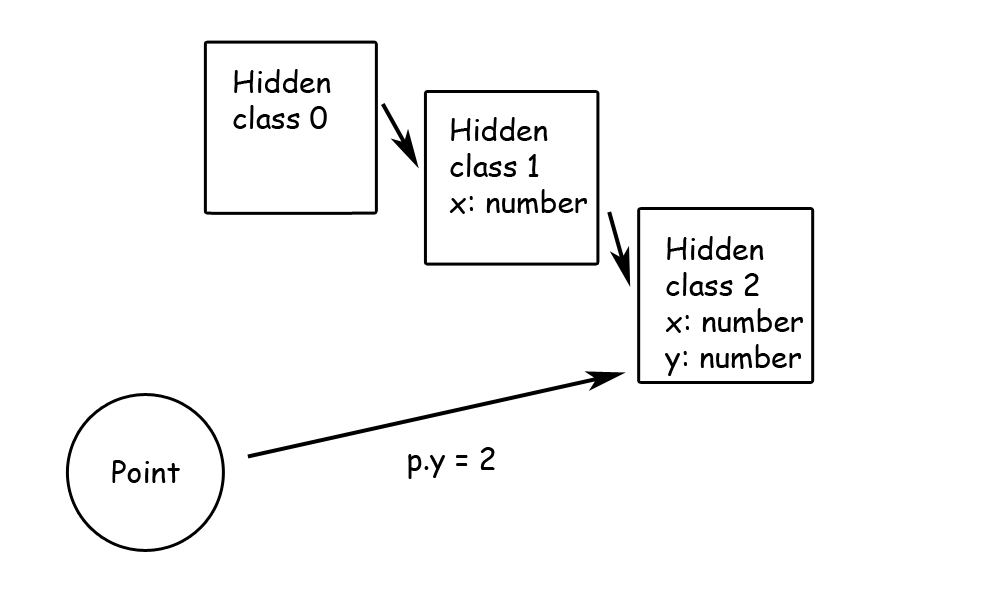
\includegraphics[width=8cm]{point2}
\end{figure}

Based on hidden class further JIT compiler optimises methods, to generate even simpler assembly code similar to one compiled from C++. Class shape defines address offsets of Object properties. Thus, hidden class graph is actually a tree, where one class can't be reached in more than one way.

\begin{figure}[h!]
  \caption{Two point representations based on order of declared properties}
  \label{img:point_tree2}
  \centering
	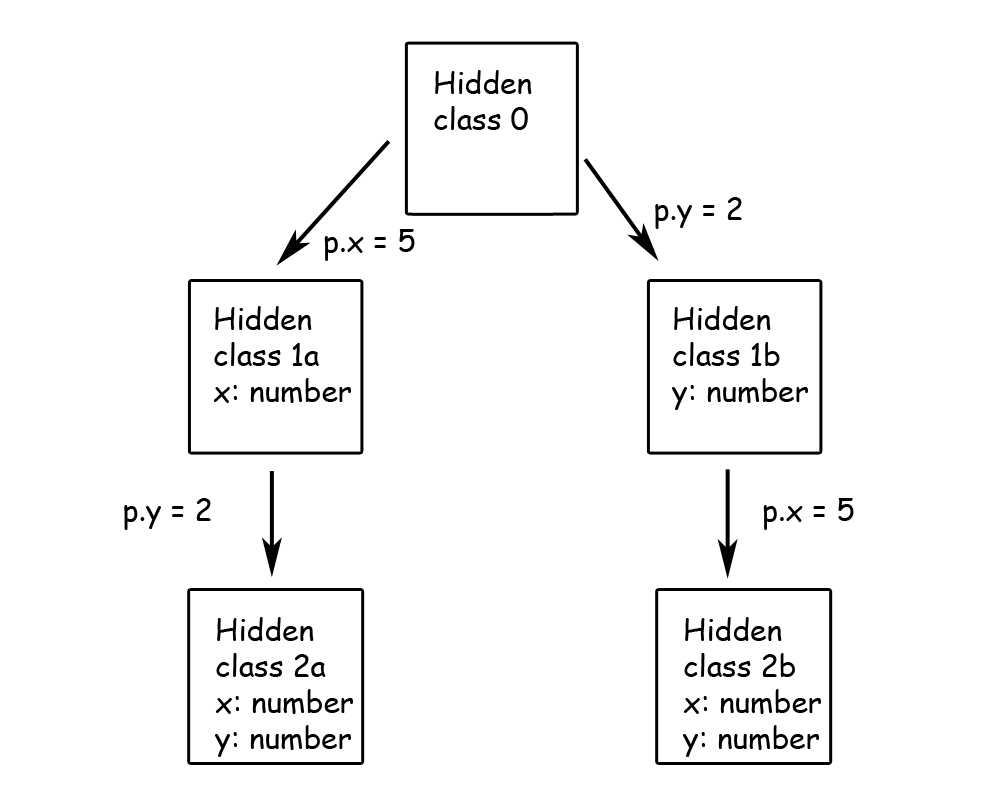
\includegraphics[width=8cm]{point_tree2}
\end{figure} 

At the moment of writing type of property is not tracked in hidden classes. The only exception are primitive values (see Listing \ref{listing:typestree}). In other words, storing an object in property results in the same hidden class regardless of hidden class of this object.

Transitions between hidden classes can be tracked in V8 using flags --trace-generalization tracking when variables are casted to more generic type (e.g. SMI to Integer, or Integer to Number) and --trace-migration (tracking when hidden classes are migrated).

\lstinputlisting[caption=Log of migration trace in V8,label=listing:migration]{migration.txt}

\section{Garbage collection}
\label{sec:garbagecollection}

Memory in JavaScript is managed automatically. Each allocation puts an object on memory heap. First generation of garbage collection traversed the whole tree and freed memory for all inaccessible objects. This type of deallocation is called mark-sweep and is causing taking a long time. Since JavaScript is single-threaded, this operation is blocking all other operations. To improve performance, especially in games, incremental scavange method of garbage collection was introduced. Engine tracks age of objects, allowing to quickly detect objects allocated temporarily (e.g. for a single frame rendered in game). When object is inaccessible, it's queued for deallocation, in chunks that don't cause long UI freezes. \footnote{http://en.wikipedia.org/wiki/Cheney's\_algorithm} \footnote{http://en.wikipedia.org/wiki/Garbage\_collection\_(computer\_science)}

TODO: check and extent

\lstinputlisting[caption=Log of garbage collection in V8,label=listing:gc]{gc.txt}
